\documentclass[10pt,a4paper,oneside]{article}
\usepackage[utf8]{inputenc}
\usepackage[english]{babel}
\usepackage{amsmath}
\usepackage{amsfonts}
\usepackage{amssymb}
\usepackage{graphicx}
%personal preferences for hyperlinks 
\usepackage[hidelinks]{hyperref}
\hypersetup{colorlinks=true}
%changing the separator before a figure's caption
\usepackage[labelsep=space]{caption}

\usepackage{url}
\usepackage{placeins}

%added to allow for spaces to be added to paths and url's
\makeatletter
\begingroup \lccode`+=32 \lowercase
 {\endgroup \def\Url@ObeySp{\Url@Edit\Url@String{ }{+}}}
 \def\Url@space{\penalty\Url@sppen\ }
\makeatother

%change font
\usepackage[T1]{fontenc}
\renewcommand{\familydefault}{\sfdefault} %computer modern sans serif

%changing the margins 
\usepackage[left=2.5cm, top=2.5cm,right=2.5cm, bottom=2.5cm]{geometry}
 \tolerance=100000  % all 3 of these commands make LaTeX less fussy about what
\hbadness=10000  % is a "good'' length/width/height of a page
\raggedbottom

%I did not find a reason why Latex was creating a blank page at the begining 
%this fixes it
\usepackage{atbegshi}% http://ctan.org/pkg/atbegshi
\AtBeginDocument{\AtBeginShipoutNext{\AtBeginShipoutDiscard}}

%document title, no date 	
\title{Windows installation guide for Abaqus 2017}
\date{}

\begin{document}
\textbf{\maketitle}
\section{Licensing notes}
Before installing Abaqus make sure you have read and understood the license requirements, in particular noting:
\begin{itemize}
\item Only appropriate authorised support staff may make physical copies of the software or documentation. 
\item Abaqus might only be installed on computers owned by the University of Sheffield, it might not be installed on computers owned by staff or students
\end{itemize}

\section{Supported compilers for Abaqus 2017}
Before you install the C/C++ and Fortran compilers you need to make sure you have a supported version of Microsoft Visual Studio as this links the compiled code with the required libraries to be used with the Abaqus solver.

Please note that the recommended Visual Studio version is VS2012 as some libraries have been redefined in the 2015 version (\url{https://msdn.microsoft.com/en-us/library/bb531344.aspx#BK_CRT}).

If you want to use a different VS version it should be done at your own discretion. Visual Studio 2015 Community Edition can be downloaded for free from the \href{https://www.Microsoft.com/en-us/download}{Microsoft download centre}).  
If you already have another version of Microsoft Visual Studio installed you can still have VS 2015 installed alongside.
You can use the Community, Professional or Enterprise edition, but \textbf{not} the Express edition as this will not work along with Abaqus. 

If you require to implement user subroutines you need to have the Intel Fortran compilers before installing Abaqus.
Intel Fortran Compiler XE 2016 Update 1 (available at the University of  Sheffield \href{https://cics.dept.shef.ac.uk/software/}{Software download service}.

For detailed information on the system prerequisites and supported platforms visit \href{http://media.3ds.com/support/progdir/all/?pdir=simulia,ep617,update00_1&context=onpremises}{3D Simulia}. For information on compatible versions of Visual Studio and Intel C/C++/Fortran compilers visit the \href{https://software.intel.com/en-us/articles/troubleshooting-fortran-integration-issues-with-visual-studio}{Intel Developer Zone} website.

\section{Microsoft Parallel Processing Interface}
The correct version of the msmpi needs to be installed on your computer so that you can successfully link your subroutines. It is always available with your Abaqus installation media and you MUST ensure you are running on the version provided by the Abaqus installation. You should not use a newer/older version as  the linker looks for the specific version given. If the wrong version is used the following error will be raised during linking: \textbf{LINK: fatal error LNK1181: cannot open input file  msmpi.lin}

If MS MPI is not present on a system, 5.0 will be automatically installed with Abaqus.

\section{Installation}
There are 4 installers which need to be run in the following order:
\begin{enumerate}
\item Abaqus documentation (optional)
\item Abaqus Services (solvers)
\item CAA developer software
\item Abaqus/CAE (interactive GUI)
\end{enumerate}

(Note you can also install Tosca and Isight using the Abaqus installer).
\\
When you start the installer, you can choose which product or products to install. Once you have made this selection, individual installers will run for each product. Most defaults values are given and it is recommended that you accept those values. Required changes will be specified in this guide. \bigskip

\textbf{Important:} you must always install both the Abaqus services (solvers) and Abaqus/CAE. They cannot be installed separately or individually.

\bigskip
Mount the iso image. To start the suite installer, right-click and select \textbf{Run as administrator} on the setup.exe file located on \path{<donwloadir>\Abaqus2017\1\setup.exe}

Once the Installer has started select the components you want to install and click Next (Fig. \ref{fig:abaqus1}).
\begin{figure}[h]
\centering
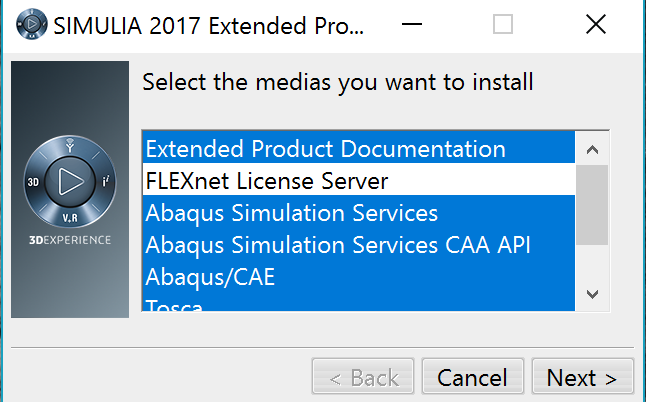
\includegraphics[width=8cm]{installer1.png} 
\caption{}
\label{fig:abaqus1}
\end{figure}
Please note you do not need installing the Flexnet license server as you will be using the University of Sheffield license server.

Separate individual installers will be launched for the different product, one after the other.

\subsection{Documentation (optional)}
The documentation installation is optional. Nonetheless it is highly recommended that you install the Abaqus documentation.

Once the installation has finished you can immediately access the documentation by opening:
 \path{C:\Program Files\Dassault Systemes\SIMULIA2017doc\DSSIMULIA_Established_homepage_English.html} in your web browser.

\subsection{Abaqus services (solvers)}
The following services are available:
\begin{itemize}
\item  Abaqus/Explicit Solver
\item Abaqus/Standard Solver
\item Cosimulation Services
\item ODB API Services
\end{itemize}
It is advisable that you install all the solvers unless you are absolutely sure you will not need one of the components. 


\subsection{Abaqus CAE}
Once the installer is running it will ask for you to select the type of license server for Abaqus. Choose FlexNet as the license type and enter the licenser server: \textbf{27000@abaquslm.shef.ac.uk} (Fig. \ref{fig:abaqus2})

\begin{figure}[ht]
\centering
	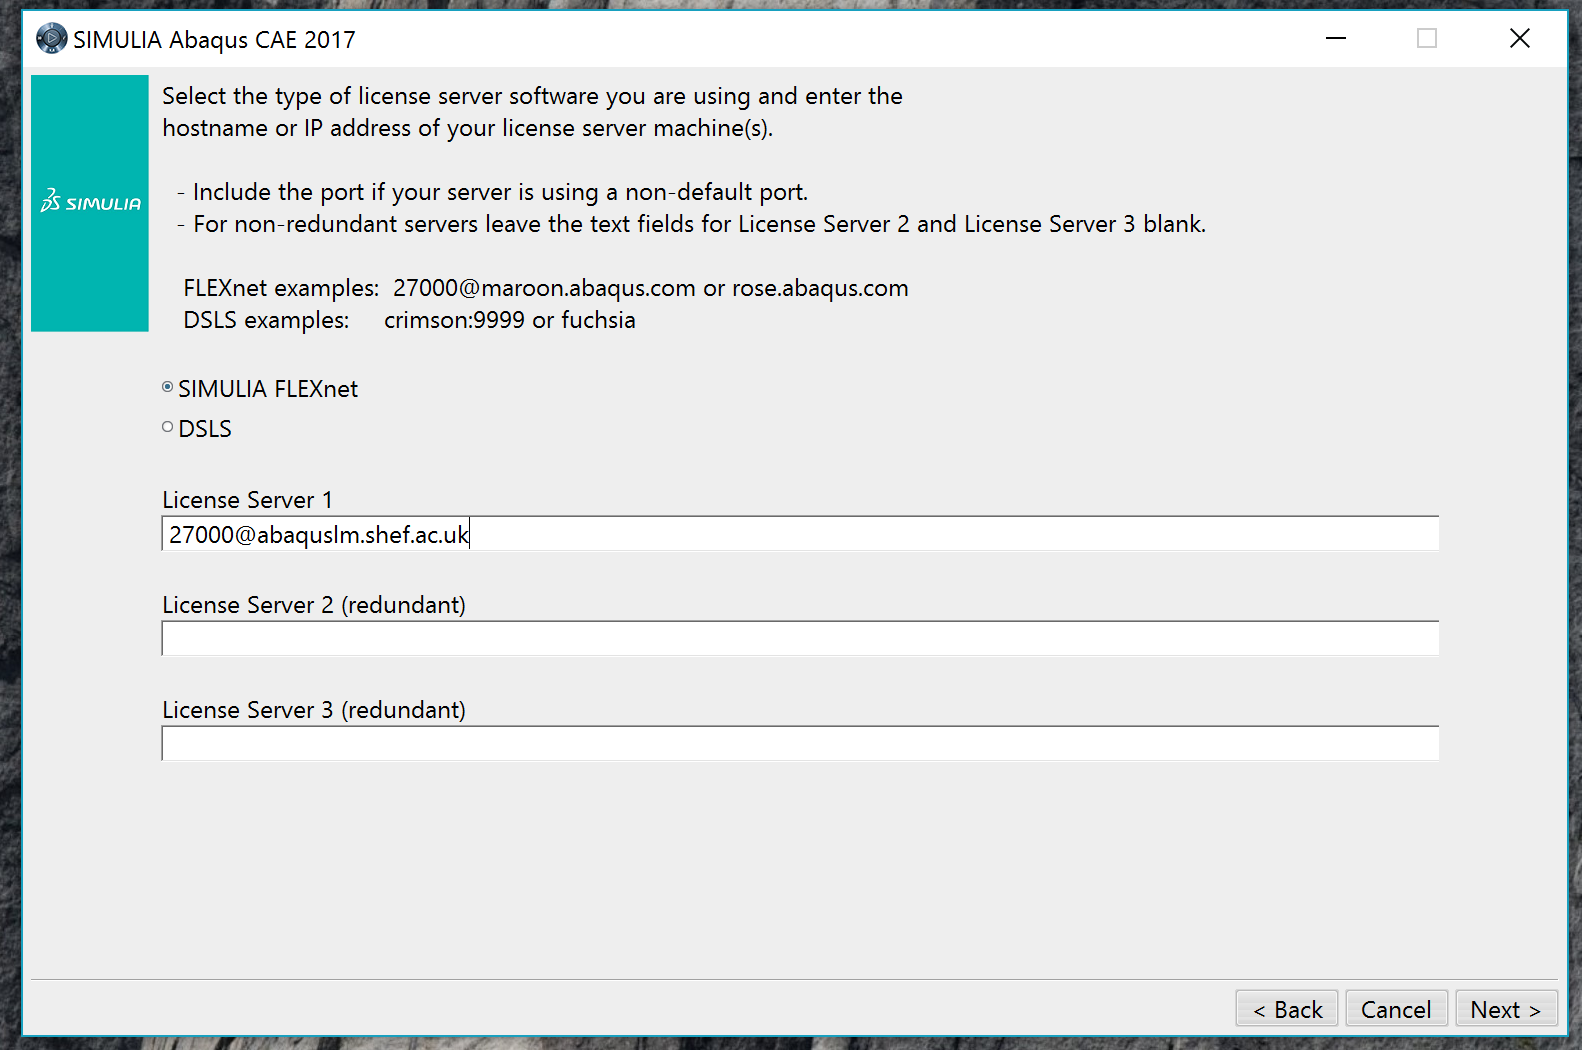
\includegraphics[width=14 cm, height=10 cm]{abaqus_license.png} 
	\caption{}
	\label{fig:abaqus2}
\end{figure}

When prompted to provide a location for the documentation select the path to your locally installed documentation. Alternatively, the URL for the served documentation can be found in \url{http://50.16.225.63} 

\textbf{Note}: the served documentation supports Abaqus versions 6.14, 2016 and 2017. If you want to directly point to the 2017 version documentation you need to go to \url{http://50.16.225.63} and log in directly to the 2917 version using your DS passport account (Fig. \ref{fig:abaqus3}).

\begin{figure}[ht]
\centering
	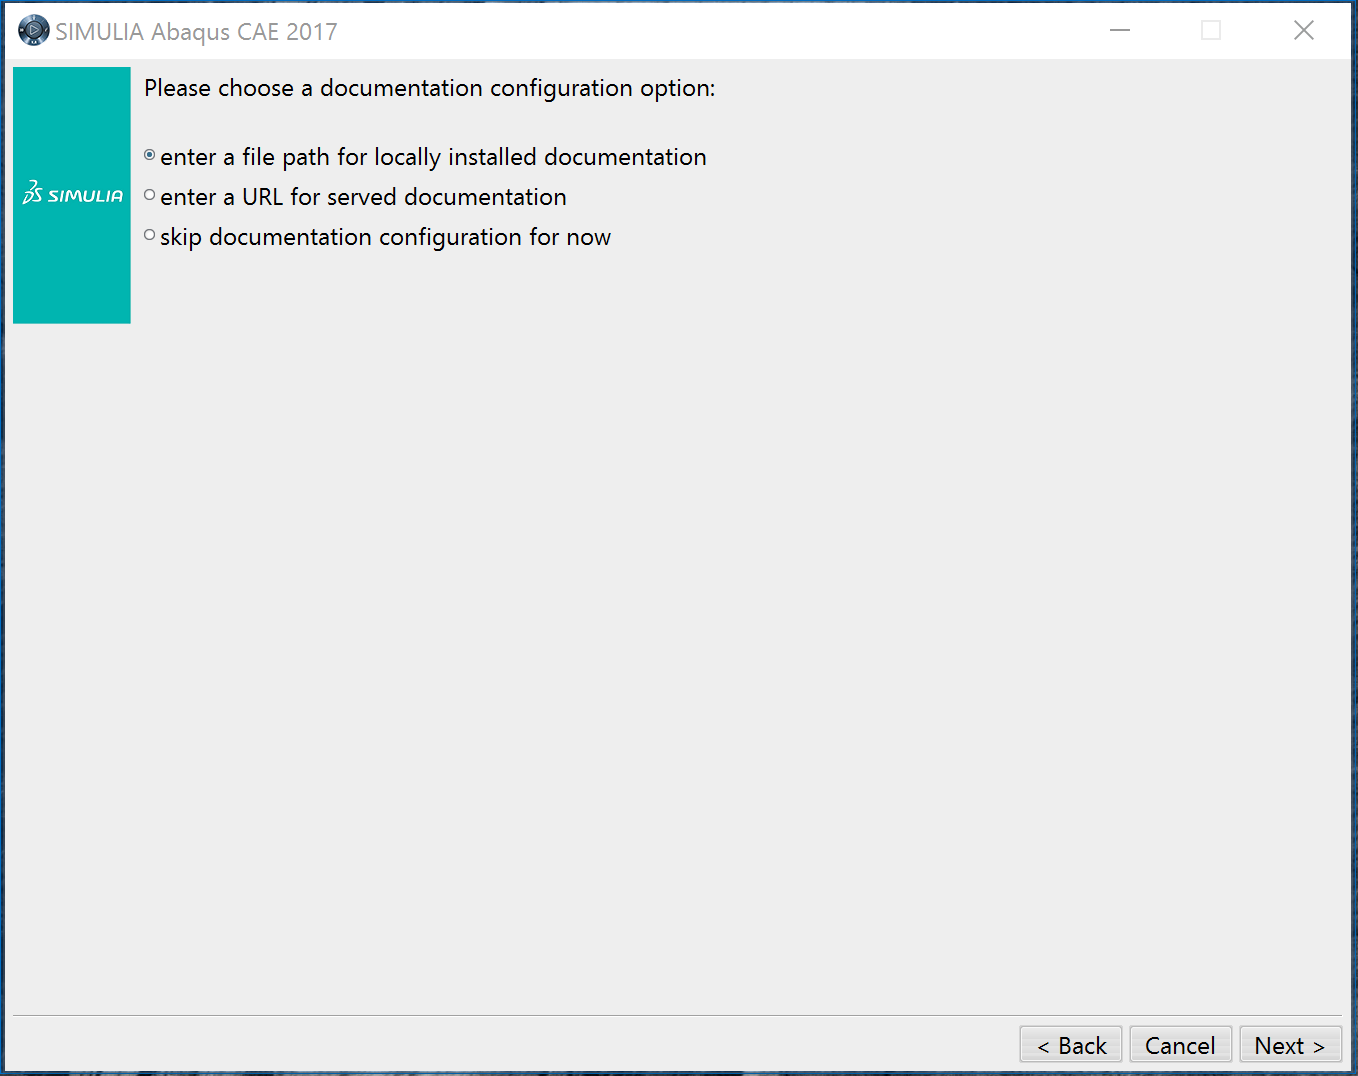
\includegraphics[width=14cm, height=10cm]{documentation_CAE.png} 
	\caption{}
	\label{fig:abaqus3}
\end{figure}
\FloatBarrier
You will be asked to choose the location of you default working directory. By default this is \textbf{\path{C:\temp}} which will be created if it does not exist. If you want to choose a different location you must ensure this directory  exists. 

\section{Verification suite}
After Abaqus CAE has been installed a verification suite will be run and the results will be displayed. This is only a sub-set of the verification suite, so it is advisable that the verification is run after installation again. 

If you need to work with subroutines you need to complete the Post-Installation tasks detailed below before running the verification again.

\section{Post-installation tasks}
\subsection{Path/short-cuts modification for subroutines} \label{sec:path}
Please note that the instructions detailed here are based on VS2012 so the paths and variables should be changed accordingly for other VS versions.

To get user subroutines working with the Intel Compiler XE 2016, copy the .bat file: \path{<donwloadir>\Abaqus2017\abaqus_set_env.bat} to your local directory: \path{C:\SIMULIA} and modify the Abaqus start menu short cuts:

\textbf{In Windows 8 and 10:}
\begin{enumerate}
\item Go to \textbf{Start menu $\rightarrow$ Dassault Systemes SIMULIA Abaqus CAE 2017}, left click on \textbf{Abaqus CAE} then right click on \textbf{More $\rightarrow$ Open file location}.
\item Once the appropriate folder is open right click on Abaqus CAE and then left click on \textbf{Properties}. 
\item Copy and paste the string below to the very beginning of the \textbf{Target} field. Ensure there is a space on either side of the \textbf{\&\&}:\\
\textbf{\path{C:\SIMULIA\abaqus_set_env.bat && }} (Fig. \ref{fig:CAEpath})
\item Repeat steps 2-3 for the Abaqus Command and Abaqus Verification short cuts in the folder.
\end{enumerate}

\textbf{In Windows 7:}
\begin{enumerate}
\item Go to \textbf{Start menu $\rightarrow$ Dassault Systemes SIMULIA Abaqus CAE 2017}, left click on \textbf{Abaqus CAE} then right click on \textbf{Properties}.
\item Copy and paste the string below to the very beginning of the \textbf{Target} field. Ensure there is a space on either side of the \textbf{\&\&}:\\
\textbf{\path{C:\SIMULIA\abaqus_set_env.bat && }}
\item Repeat the above steps for the Abaqus Command and Abaqus Verification short cuts in the folder.
\end{enumerate}

\begin{figure}[!h]
\centering
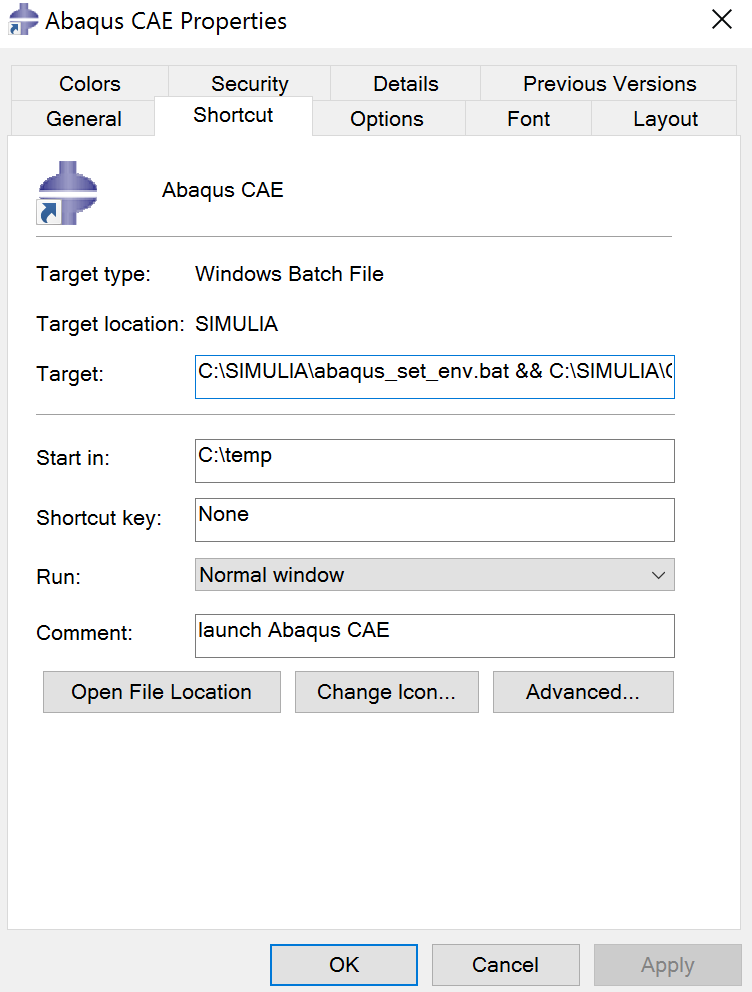
\includegraphics[scale=0.7]{abaqus_CAE.png} 
\caption{}
\label{fig:CAEpath}
\end{figure}

\subsection{Manual configuration}
Note that the "\path{abaqus_set_env.bat}" file calls the various compilers and dependencies needed for to compile the Fortran subroutines. If you changed the default installation location for Visual Studio or Intel XE Composer  you need to amend the paths in the .bat file. 

If you prefer to manually add the compilers paths to Abaqus CAE, command, and verification you first need to find the location of your Fortran compilers which should look something like this: 

%\bigbreak
%\path{C:\Program Files (x86)\IntelSWTools\compilers_and_libraries_2016.1.146}\newline
%\path{\windows\bin\ipsxe-comp-vars.bat} 
%\bigbreak
\path{C:\Program Files (x86)\IntelSWTools\compilers_and_libraries_2016.1.146}\newline
\path{\windows\bin\ifortvars.bat}
\bigbreak

You will then need to pass these paths directly to Abaqus along with the VS Studio version you are running. Follow the steps indicated in the above section (sec. \ref{sec:path}). Instead of adding the path to the "\path{abaqus_set_env.bat}" file  you need to add the paths to your compilers location. The corresponding Targets should look something like this:

\begin{itemize}
\item \textbf{Abaqus CAE }\\
%\path{"C:\Program Files (x86)\IntelSWTools\compilers_and_libraries_2016.1.146\windows} \newline 
%\path{\bin\ipsxe-comp-vars.bat" intel64 vs 2015 && 

\path{"C:\Program Files (x86)\IntelSWTools\compilers_and_libraries_2016.1.146\windows\bin\ifortvars.bat" intel64 vs2012 && C:\SIMULIA\Commands\abaqus2017.bat cae || pause}
\item \textbf{Abaqus Command }\\
%\path{"C:\Program Files (x86)\IntelSWTools\compilers_and_libraries_2016.1.146\windows} \newline 
%\path{\bin\ipsxe-comp-vars.bat" intel64 vs 2015 && 
\path{"C:\Program Files (x86)\IntelSWTools\compilers_and_libraries_2016.1.146\windows\bin\ifortvars.bat" intel64 vs2012 && C:\Windows\SysWOW64\cmd.exe /k}
\item \textbf{Abaqus Verification }\\
%\path{"C:\Program Files (x86)\IntelSWTools\compilers_and_libraries_2016.1.146\windows} \newline 
%\path{\bin\ipsxe-comp-vars.bat" intel64 vs 2015 && 
\path{"C:\Program Files (x86)\IntelSWTools\compilers_and_libraries_2016.1.146\windows\bin\ifortvars.bat" intel64 vs2012 && } \newline 
\path{C:\SIMULIA\CAE\2016\win_b64\resources\install\cae\launcher.bat -verify -all -log && notepad.exe
verify.log || notepad.exe verify.log}
\end{itemize}

Once again make sure there is a space on either side of the \textbf{\&\&}, also note the " " included as the paths have spaces. 

\subsection{Set your environment variables}
\begin{enumerate}
\item Double-click on the \textbf{vcvarsall.bat} file, which should be found on a path similar to\\
\path{C:\Program Files (x86)\Microsoft Visual Studio 11.0\VC\vcvasrsall.bat}
\item Double-click on the \textbf{ifortvars.bat} file, which should be found on a path similar to\\
\path{C:\Program Files (x86)\IntelSWTools\compilers_and_libraries_2016.1.146\windows\bin\ifortvars.bat}
\item Open an Abaqus command prompt and type \textbf{set>path.info}
\item Open the generated path.info file (located in your default Abaqus working directory e.g. \path{C:\temp}).
\item Locate the variables for "path", "lib", and "include"
\item Then go to \textbf{Start menu} $\rightarrow$ \textbf{Control Panel} $\rightarrow$ \textbf{Sytem} $\rightarrow$ \textbf{Advanced system settings} (Note you need admin rights for this).
\item Click on \textbf{Environment variables} and under the \textbf{System variables}, progressively select each of the environment variables \textbf{path, lib,} and \textbf{ include}. For each variable click \textbf{edit} and replace the variable with the entire string of pathnames from the \textbf{path.info} file. Make sure you do not have duplicated pathnames and that each variable has a semi-colon after each pathname. Click \textbf{OK} and then \textbf{OK}.
\end{enumerate}

Note that in some cases you might need to restart your computer for the changes to take effect.

\subsection{Full verification}
After completing the configuration for Abaqus subroutines run the verification suite to test the installation. 
Start Menu $\rightarrow$ Dassault Systemes SIMULIA Abaqus 2017 $\rightarrow$ Abaqus Verification.

A series of tests will be run automatically, the tests should then be reported as PASS in the verify.log file. If Abaqus has not been correctly configured to run Fortran subroutines and C++ compilers then the corresponding tests will fail and you will prompted to look at the log file for the failed test.
 
 If the compilation of the Fortran subroutine fails, it is possible that there exist some integration issues between Fortran and Visual Studio. Please refer to this page in the \href{https://software.intel.com/en-us/articles/troubleshooting-fortran-integration-issues-with-visual-studio}{Intel Developer Zone} for integration issues troubleshooting.
\end{document}

Alternatively, you can only test for the standard user subroutines by launching an Abaqus command prompt and type: \textbf{"abaqus verify -user_std"}. This will only verify the user subroutines and the results will be stored in your default working directory. Check that every test passes.

If you get a legend \textbf{"ifort not recognised as an internal or external operator"} it indicates that the paths to your Fortran compilers were not set correctly, make sure you followed the above instructions correctly. 

If you get a legend \textbf{"Abaqus user subroutines library could not be found"} it might indicate that your Abaqus installation was not done correctly. 




